% Created by tikzDevice version 0.12.3.1 on 2023-04-12 15:06:51
% !TEX encoding = UTF-8 Unicode
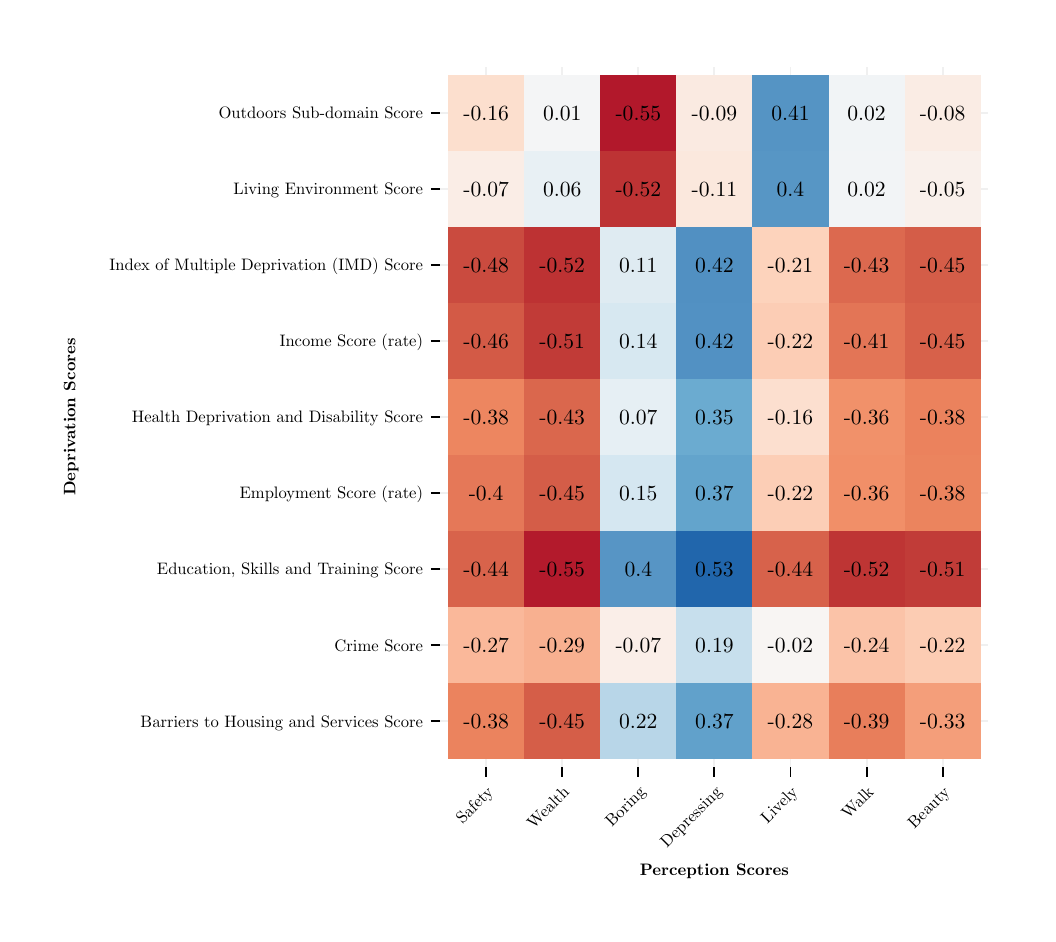
\begin{tikzpicture}[x=1pt,y=1pt]
\definecolor{fillColor}{RGB}{255,255,255}
\begin{scope}
\definecolor{fillColor}{RGB}{255,255,255}

\path[fill=fillColor] (  0.00, 20.54) rectangle (361.35,340.81);
\end{scope}
\begin{scope}
\definecolor{fillColor}{RGB}{255,255,255}

\path[fill=fillColor] (149.17, 73.65) rectangle (347.12,326.58);
\definecolor{drawColor}{gray}{0.94}

\path[draw=drawColor,line width= 0.7pt,line join=round] (149.17, 90.14) --
	(347.12, 90.14);

\path[draw=drawColor,line width= 0.7pt,line join=round] (149.17,117.64) --
	(347.12,117.64);

\path[draw=drawColor,line width= 0.7pt,line join=round] (149.17,145.13) --
	(347.12,145.13);

\path[draw=drawColor,line width= 0.7pt,line join=round] (149.17,172.62) --
	(347.12,172.62);

\path[draw=drawColor,line width= 0.7pt,line join=round] (149.17,200.12) --
	(347.12,200.12);

\path[draw=drawColor,line width= 0.7pt,line join=round] (149.17,227.61) --
	(347.12,227.61);

\path[draw=drawColor,line width= 0.7pt,line join=round] (149.17,255.10) --
	(347.12,255.10);

\path[draw=drawColor,line width= 0.7pt,line join=round] (149.17,282.60) --
	(347.12,282.60);

\path[draw=drawColor,line width= 0.7pt,line join=round] (149.17,310.09) --
	(347.12,310.09);

\path[draw=drawColor,line width= 0.7pt,line join=round] (165.67, 73.65) --
	(165.67,326.58);

\path[draw=drawColor,line width= 0.7pt,line join=round] (193.16, 73.65) --
	(193.16,326.58);

\path[draw=drawColor,line width= 0.7pt,line join=round] (220.66, 73.65) --
	(220.66,326.58);

\path[draw=drawColor,line width= 0.7pt,line join=round] (248.15, 73.65) --
	(248.15,326.58);

\path[draw=drawColor,line width= 0.7pt,line join=round] (275.64, 73.65) --
	(275.64,326.58);

\path[draw=drawColor,line width= 0.7pt,line join=round] (303.13, 73.65) --
	(303.13,326.58);

\path[draw=drawColor,line width= 0.7pt,line join=round] (330.63, 73.65) --
	(330.63,326.58);
\definecolor{fillColor}{RGB}{250,237,230}

\path[fill=fillColor] (151.92,268.85) rectangle (179.42,296.34);
\definecolor{fillColor}{RGB}{250,184,154}

\path[fill=fillColor] (151.92,103.89) rectangle (179.42,131.38);
\definecolor{fillColor}{RGB}{237,134,96}

\path[fill=fillColor] (151.92,186.37) rectangle (179.42,213.86);
\definecolor{fillColor}{RGB}{235,131,94}

\path[fill=fillColor] (151.92, 76.40) rectangle (179.42,103.89);
\definecolor{fillColor}{RGB}{216,99,75}

\path[fill=fillColor] (151.92,131.38) rectangle (179.42,158.88);
\definecolor{fillColor}{RGB}{229,120,88}

\path[fill=fillColor] (151.92,158.88) rectangle (179.42,186.37);
\definecolor{fillColor}{RGB}{211,90,70}

\path[fill=fillColor] (151.92,213.86) rectangle (179.42,241.36);
\definecolor{fillColor}{RGB}{202,75,63}

\path[fill=fillColor] (151.92,241.36) rectangle (179.42,268.85);
\definecolor{fillColor}{RGB}{252,223,206}

\path[fill=fillColor] (151.92,296.34) rectangle (179.42,323.84);
\definecolor{fillColor}{RGB}{232,240,244}

\path[fill=fillColor] (179.42,268.85) rectangle (206.91,296.34);
\definecolor{fillColor}{RGB}{248,176,144}

\path[fill=fillColor] (179.42,103.89) rectangle (206.91,131.38);
\definecolor{fillColor}{RGB}{218,103,77}

\path[fill=fillColor] (179.42,186.37) rectangle (206.91,213.86);
\definecolor{fillColor}{RGB}{213,94,72}

\path[fill=fillColor] (179.42, 76.40) rectangle (206.91,103.89);
\definecolor{fillColor}{RGB}{179,26,44}

\path[fill=fillColor] (179.42,131.38) rectangle (206.91,158.88);
\definecolor{fillColor}{RGB}{212,93,72}

\path[fill=fillColor] (179.42,158.88) rectangle (206.91,186.37);
\definecolor{fillColor}{RGB}{193,59,55}

\path[fill=fillColor] (179.42,213.86) rectangle (206.91,241.36);
\definecolor{fillColor}{RGB}{189,50,51}

\path[fill=fillColor] (179.42,241.36) rectangle (206.91,268.85);
\definecolor{fillColor}{RGB}{244,245,246}

\path[fill=fillColor] (179.42,296.34) rectangle (206.91,323.84);
\definecolor{fillColor}{RGB}{189,51,52}

\path[fill=fillColor] (206.91,268.85) rectangle (234.40,296.34);
\definecolor{fillColor}{RGB}{250,238,232}

\path[fill=fillColor] (206.91,103.89) rectangle (234.40,131.38);
\definecolor{fillColor}{RGB}{230,239,244}

\path[fill=fillColor] (206.91,186.37) rectangle (234.40,213.86);
\definecolor{fillColor}{RGB}{184,214,232}

\path[fill=fillColor] (206.91, 76.40) rectangle (234.40,103.89);
\definecolor{fillColor}{RGB}{87,149,197}

\path[fill=fillColor] (206.91,131.38) rectangle (234.40,158.88);
\definecolor{fillColor}{RGB}{213,231,241}

\path[fill=fillColor] (206.91,158.88) rectangle (234.40,186.37);
\definecolor{fillColor}{RGB}{215,232,241}

\path[fill=fillColor] (206.91,213.86) rectangle (234.40,241.36);
\definecolor{fillColor}{RGB}{223,235,242}

\path[fill=fillColor] (206.91,241.36) rectangle (234.40,268.85);
\definecolor{fillColor}{RGB}{178,24,43}

\path[fill=fillColor] (206.91,296.34) rectangle (234.40,323.84);
\definecolor{fillColor}{RGB}{251,232,221}

\path[fill=fillColor] (234.40,268.85) rectangle (261.90,296.34);
\definecolor{fillColor}{RGB}{199,223,237}

\path[fill=fillColor] (234.40,103.89) rectangle (261.90,131.38);
\definecolor{fillColor}{RGB}{107,171,208}

\path[fill=fillColor] (234.40,186.37) rectangle (261.90,213.86);
\definecolor{fillColor}{RGB}{97,161,203}

\path[fill=fillColor] (234.40, 76.40) rectangle (261.90,103.89);
\definecolor{fillColor}{RGB}{33,102,172}

\path[fill=fillColor] (234.40,131.38) rectangle (261.90,158.88);
\definecolor{fillColor}{RGB}{99,164,204}

\path[fill=fillColor] (234.40,158.88) rectangle (261.90,186.37);
\definecolor{fillColor}{RGB}{82,145,195}

\path[fill=fillColor] (234.40,213.86) rectangle (261.90,241.36);
\definecolor{fillColor}{RGB}{81,144,194}

\path[fill=fillColor] (234.40,241.36) rectangle (261.90,268.85);
\definecolor{fillColor}{RGB}{250,234,225}

\path[fill=fillColor] (234.40,296.34) rectangle (261.90,323.84);
\definecolor{fillColor}{RGB}{87,150,197}

\path[fill=fillColor] (261.90,268.85) rectangle (289.39,296.34);
\definecolor{fillColor}{RGB}{248,245,243}

\path[fill=fillColor] (261.90,103.89) rectangle (289.39,131.38);
\definecolor{fillColor}{RGB}{252,223,207}

\path[fill=fillColor] (261.90,186.37) rectangle (289.39,213.86);
\definecolor{fillColor}{RGB}{249,179,147}

\path[fill=fillColor] (261.90, 76.40) rectangle (289.39,103.89);
\definecolor{fillColor}{RGB}{215,98,75}

\path[fill=fillColor] (261.90,131.38) rectangle (289.39,158.88);
\definecolor{fillColor}{RGB}{252,206,182}

\path[fill=fillColor] (261.90,158.88) rectangle (289.39,186.37);
\definecolor{fillColor}{RGB}{252,205,181}

\path[fill=fillColor] (261.90,213.86) rectangle (289.39,241.36);
\definecolor{fillColor}{RGB}{253,211,188}

\path[fill=fillColor] (261.90,241.36) rectangle (289.39,268.85);
\definecolor{fillColor}{RGB}{85,148,196}

\path[fill=fillColor] (261.90,296.34) rectangle (289.39,323.84);
\definecolor{fillColor}{RGB}{242,244,246}

\path[fill=fillColor] (289.39,268.85) rectangle (316.88,296.34);
\definecolor{fillColor}{RGB}{251,195,168}

\path[fill=fillColor] (289.39,103.89) rectangle (316.88,131.38);
\definecolor{fillColor}{RGB}{241,145,106}

\path[fill=fillColor] (289.39,186.37) rectangle (316.88,213.86);
\definecolor{fillColor}{RGB}{232,126,91}

\path[fill=fillColor] (289.39, 76.40) rectangle (316.88,103.89);
\definecolor{fillColor}{RGB}{190,53,52}

\path[fill=fillColor] (289.39,131.38) rectangle (316.88,158.88);
\definecolor{fillColor}{RGB}{241,143,104}

\path[fill=fillColor] (289.39,158.88) rectangle (316.88,186.37);
\definecolor{fillColor}{RGB}{227,117,86}

\path[fill=fillColor] (289.39,213.86) rectangle (316.88,241.36);
\definecolor{fillColor}{RGB}{220,105,79}

\path[fill=fillColor] (289.39,241.36) rectangle (316.88,268.85);
\definecolor{fillColor}{RGB}{241,244,246}

\path[fill=fillColor] (289.39,296.34) rectangle (316.88,323.84);
\definecolor{fillColor}{RGB}{249,240,235}

\path[fill=fillColor] (316.88,268.85) rectangle (344.37,296.34);
\definecolor{fillColor}{RGB}{252,204,179}

\path[fill=fillColor] (316.88,103.89) rectangle (344.37,131.38);
\definecolor{fillColor}{RGB}{235,130,93}

\path[fill=fillColor] (316.88,186.37) rectangle (344.37,213.86);
\definecolor{fillColor}{RGB}{244,158,122}

\path[fill=fillColor] (316.88, 76.40) rectangle (344.37,103.89);
\definecolor{fillColor}{RGB}{193,60,56}

\path[fill=fillColor] (316.88,131.38) rectangle (344.37,158.88);
\definecolor{fillColor}{RGB}{235,132,94}

\path[fill=fillColor] (316.88,158.88) rectangle (344.37,186.37);
\definecolor{fillColor}{RGB}{215,97,74}

\path[fill=fillColor] (316.88,213.86) rectangle (344.37,241.36);
\definecolor{fillColor}{RGB}{212,93,72}

\path[fill=fillColor] (316.88,241.36) rectangle (344.37,268.85);
\definecolor{fillColor}{RGB}{250,236,228}

\path[fill=fillColor] (316.88,296.34) rectangle (344.37,323.84);
\definecolor{drawColor}{RGB}{0,0,0}

\node[text=drawColor,anchor=base,inner sep=0pt, outer sep=0pt, scale=  0.78] at (165.67,279.90) {-0.07};

\node[text=drawColor,anchor=base,inner sep=0pt, outer sep=0pt, scale=  0.78] at (165.67,114.94) {-0.27};

\node[text=drawColor,anchor=base,inner sep=0pt, outer sep=0pt, scale=  0.78] at (165.67,197.42) {-0.38};

\node[text=drawColor,anchor=base,inner sep=0pt, outer sep=0pt, scale=  0.78] at (165.67, 87.45) {-0.38};

\node[text=drawColor,anchor=base,inner sep=0pt, outer sep=0pt, scale=  0.78] at (165.67,142.44) {-0.44};

\node[text=drawColor,anchor=base,inner sep=0pt, outer sep=0pt, scale=  0.78] at (165.67,169.93) {-0.4};

\node[text=drawColor,anchor=base,inner sep=0pt, outer sep=0pt, scale=  0.78] at (165.67,224.92) {-0.46};

\node[text=drawColor,anchor=base,inner sep=0pt, outer sep=0pt, scale=  0.78] at (165.67,252.41) {-0.48};

\node[text=drawColor,anchor=base,inner sep=0pt, outer sep=0pt, scale=  0.78] at (165.67,307.39) {-0.16};

\node[text=drawColor,anchor=base,inner sep=0pt, outer sep=0pt, scale=  0.78] at (193.16,279.90) {0.06};

\node[text=drawColor,anchor=base,inner sep=0pt, outer sep=0pt, scale=  0.78] at (193.16,114.94) {-0.29};

\node[text=drawColor,anchor=base,inner sep=0pt, outer sep=0pt, scale=  0.78] at (193.16,197.42) {-0.43};

\node[text=drawColor,anchor=base,inner sep=0pt, outer sep=0pt, scale=  0.78] at (193.16, 87.45) {-0.45};

\node[text=drawColor,anchor=base,inner sep=0pt, outer sep=0pt, scale=  0.78] at (193.16,142.44) {-0.55};

\node[text=drawColor,anchor=base,inner sep=0pt, outer sep=0pt, scale=  0.78] at (193.16,169.93) {-0.45};

\node[text=drawColor,anchor=base,inner sep=0pt, outer sep=0pt, scale=  0.78] at (193.16,224.92) {-0.51};

\node[text=drawColor,anchor=base,inner sep=0pt, outer sep=0pt, scale=  0.78] at (193.16,252.41) {-0.52};

\node[text=drawColor,anchor=base,inner sep=0pt, outer sep=0pt, scale=  0.78] at (193.16,307.39) {0.01};

\node[text=drawColor,anchor=base,inner sep=0pt, outer sep=0pt, scale=  0.78] at (220.66,279.90) {-0.52};

\node[text=drawColor,anchor=base,inner sep=0pt, outer sep=0pt, scale=  0.78] at (220.66,114.94) {-0.07};

\node[text=drawColor,anchor=base,inner sep=0pt, outer sep=0pt, scale=  0.78] at (220.66,197.42) {0.07};

\node[text=drawColor,anchor=base,inner sep=0pt, outer sep=0pt, scale=  0.78] at (220.66, 87.45) {0.22};

\node[text=drawColor,anchor=base,inner sep=0pt, outer sep=0pt, scale=  0.78] at (220.66,142.44) {0.4};

\node[text=drawColor,anchor=base,inner sep=0pt, outer sep=0pt, scale=  0.78] at (220.66,169.93) {0.15};

\node[text=drawColor,anchor=base,inner sep=0pt, outer sep=0pt, scale=  0.78] at (220.66,224.92) {0.14};

\node[text=drawColor,anchor=base,inner sep=0pt, outer sep=0pt, scale=  0.78] at (220.66,252.41) {0.11};

\node[text=drawColor,anchor=base,inner sep=0pt, outer sep=0pt, scale=  0.78] at (220.66,307.39) {-0.55};

\node[text=drawColor,anchor=base,inner sep=0pt, outer sep=0pt, scale=  0.78] at (248.15,279.90) {-0.11};

\node[text=drawColor,anchor=base,inner sep=0pt, outer sep=0pt, scale=  0.78] at (248.15,114.94) {0.19};

\node[text=drawColor,anchor=base,inner sep=0pt, outer sep=0pt, scale=  0.78] at (248.15,197.42) {0.35};

\node[text=drawColor,anchor=base,inner sep=0pt, outer sep=0pt, scale=  0.78] at (248.15, 87.45) {0.37};

\node[text=drawColor,anchor=base,inner sep=0pt, outer sep=0pt, scale=  0.78] at (248.15,142.44) {0.53};

\node[text=drawColor,anchor=base,inner sep=0pt, outer sep=0pt, scale=  0.78] at (248.15,169.93) {0.37};

\node[text=drawColor,anchor=base,inner sep=0pt, outer sep=0pt, scale=  0.78] at (248.15,224.92) {0.42};

\node[text=drawColor,anchor=base,inner sep=0pt, outer sep=0pt, scale=  0.78] at (248.15,252.41) {0.42};

\node[text=drawColor,anchor=base,inner sep=0pt, outer sep=0pt, scale=  0.78] at (248.15,307.39) {-0.09};

\node[text=drawColor,anchor=base,inner sep=0pt, outer sep=0pt, scale=  0.78] at (275.64,279.90) {0.4};

\node[text=drawColor,anchor=base,inner sep=0pt, outer sep=0pt, scale=  0.78] at (275.64,114.94) {-0.02};

\node[text=drawColor,anchor=base,inner sep=0pt, outer sep=0pt, scale=  0.78] at (275.64,197.42) {-0.16};

\node[text=drawColor,anchor=base,inner sep=0pt, outer sep=0pt, scale=  0.78] at (275.64, 87.45) {-0.28};

\node[text=drawColor,anchor=base,inner sep=0pt, outer sep=0pt, scale=  0.78] at (275.64,142.44) {-0.44};

\node[text=drawColor,anchor=base,inner sep=0pt, outer sep=0pt, scale=  0.78] at (275.64,169.93) {-0.22};

\node[text=drawColor,anchor=base,inner sep=0pt, outer sep=0pt, scale=  0.78] at (275.64,224.92) {-0.22};

\node[text=drawColor,anchor=base,inner sep=0pt, outer sep=0pt, scale=  0.78] at (275.64,252.41) {-0.21};

\node[text=drawColor,anchor=base,inner sep=0pt, outer sep=0pt, scale=  0.78] at (275.64,307.39) {0.41};

\node[text=drawColor,anchor=base,inner sep=0pt, outer sep=0pt, scale=  0.78] at (303.13,279.90) {0.02};

\node[text=drawColor,anchor=base,inner sep=0pt, outer sep=0pt, scale=  0.78] at (303.13,114.94) {-0.24};

\node[text=drawColor,anchor=base,inner sep=0pt, outer sep=0pt, scale=  0.78] at (303.13,197.42) {-0.36};

\node[text=drawColor,anchor=base,inner sep=0pt, outer sep=0pt, scale=  0.78] at (303.13, 87.45) {-0.39};

\node[text=drawColor,anchor=base,inner sep=0pt, outer sep=0pt, scale=  0.78] at (303.13,142.44) {-0.52};

\node[text=drawColor,anchor=base,inner sep=0pt, outer sep=0pt, scale=  0.78] at (303.13,169.93) {-0.36};

\node[text=drawColor,anchor=base,inner sep=0pt, outer sep=0pt, scale=  0.78] at (303.13,224.92) {-0.41};

\node[text=drawColor,anchor=base,inner sep=0pt, outer sep=0pt, scale=  0.78] at (303.13,252.41) {-0.43};

\node[text=drawColor,anchor=base,inner sep=0pt, outer sep=0pt, scale=  0.78] at (303.13,307.39) {0.02};

\node[text=drawColor,anchor=base,inner sep=0pt, outer sep=0pt, scale=  0.78] at (330.63,279.90) {-0.05};

\node[text=drawColor,anchor=base,inner sep=0pt, outer sep=0pt, scale=  0.78] at (330.63,114.94) {-0.22};

\node[text=drawColor,anchor=base,inner sep=0pt, outer sep=0pt, scale=  0.78] at (330.63,197.42) {-0.38};

\node[text=drawColor,anchor=base,inner sep=0pt, outer sep=0pt, scale=  0.78] at (330.63, 87.45) {-0.33};

\node[text=drawColor,anchor=base,inner sep=0pt, outer sep=0pt, scale=  0.78] at (330.63,142.44) {-0.51};

\node[text=drawColor,anchor=base,inner sep=0pt, outer sep=0pt, scale=  0.78] at (330.63,169.93) {-0.38};

\node[text=drawColor,anchor=base,inner sep=0pt, outer sep=0pt, scale=  0.78] at (330.63,224.92) {-0.45};

\node[text=drawColor,anchor=base,inner sep=0pt, outer sep=0pt, scale=  0.78] at (330.63,252.41) {-0.45};

\node[text=drawColor,anchor=base,inner sep=0pt, outer sep=0pt, scale=  0.78] at (330.63,307.39) {-0.08};

\path[] (149.17, 73.65) rectangle (347.12,326.58);
\end{scope}
\begin{scope}

\path[] (149.17, 73.65) --
	(149.17,326.58);
\end{scope}
\begin{scope}
\definecolor{drawColor}{RGB}{0,0,0}

\node[text=drawColor,anchor=base east,inner sep=0pt, outer sep=0pt, scale=  0.60] at (142.87, 88.08) {Barriers to Housing and Services Score};

\node[text=drawColor,anchor=base east,inner sep=0pt, outer sep=0pt, scale=  0.60] at (142.87,115.57) {Crime Score};

\node[text=drawColor,anchor=base east,inner sep=0pt, outer sep=0pt, scale=  0.60] at (142.87,143.06) {Education, Skills and Training Score};

\node[text=drawColor,anchor=base east,inner sep=0pt, outer sep=0pt, scale=  0.60] at (142.87,170.56) {Employment Score (rate)};

\node[text=drawColor,anchor=base east,inner sep=0pt, outer sep=0pt, scale=  0.60] at (142.87,198.05) {Health Deprivation and Disability Score};

\node[text=drawColor,anchor=base east,inner sep=0pt, outer sep=0pt, scale=  0.60] at (142.87,225.54) {Income Score (rate)};

\node[text=drawColor,anchor=base east,inner sep=0pt, outer sep=0pt, scale=  0.60] at (142.87,253.04) {Index of Multiple Deprivation (IMD) Score};

\node[text=drawColor,anchor=base east,inner sep=0pt, outer sep=0pt, scale=  0.60] at (142.87,280.53) {Living Environment Score};

\node[text=drawColor,anchor=base east,inner sep=0pt, outer sep=0pt, scale=  0.60] at (142.87,308.02) {Outdoors Sub-domain Score};
\end{scope}
\begin{scope}
\definecolor{drawColor}{RGB}{0,0,0}

\path[draw=drawColor,line width= 0.7pt,line join=round] (145.67, 90.14) --
	(149.17, 90.14);

\path[draw=drawColor,line width= 0.7pt,line join=round] (145.67,117.64) --
	(149.17,117.64);

\path[draw=drawColor,line width= 0.7pt,line join=round] (145.67,145.13) --
	(149.17,145.13);

\path[draw=drawColor,line width= 0.7pt,line join=round] (145.67,172.62) --
	(149.17,172.62);

\path[draw=drawColor,line width= 0.7pt,line join=round] (145.67,200.12) --
	(149.17,200.12);

\path[draw=drawColor,line width= 0.7pt,line join=round] (145.67,227.61) --
	(149.17,227.61);

\path[draw=drawColor,line width= 0.7pt,line join=round] (145.67,255.10) --
	(149.17,255.10);

\path[draw=drawColor,line width= 0.7pt,line join=round] (145.67,282.60) --
	(149.17,282.60);

\path[draw=drawColor,line width= 0.7pt,line join=round] (145.67,310.09) --
	(149.17,310.09);
\end{scope}
\begin{scope}

\path[] (149.17, 73.65) --
	(347.12, 73.65);
\end{scope}
\begin{scope}
\definecolor{drawColor}{RGB}{0,0,0}

\path[draw=drawColor,line width= 0.7pt,line join=round] (165.67, 70.15) --
	(165.67, 73.65);

\path[draw=drawColor,line width= 0.7pt,line join=round] (193.16, 70.15) --
	(193.16, 73.65);

\path[draw=drawColor,line width= 0.7pt,line join=round] (220.66, 70.15) --
	(220.66, 73.65);

\path[draw=drawColor,line width= 0.7pt,line join=round] (248.15, 70.15) --
	(248.15, 73.65);

\path[draw=drawColor,line width= 0.7pt,line join=round] (275.64, 70.15) --
	(275.64, 73.65);

\path[draw=drawColor,line width= 0.7pt,line join=round] (303.13, 70.15) --
	(303.13, 73.65);

\path[draw=drawColor,line width= 0.7pt,line join=round] (330.63, 70.15) --
	(330.63, 73.65);
\end{scope}
\begin{scope}
\definecolor{drawColor}{RGB}{0,0,0}

\node[text=drawColor,rotate= 45.00,anchor=base east,inner sep=0pt, outer sep=0pt, scale=  0.60] at (168.56, 64.22) {Safety};

\node[text=drawColor,rotate= 45.00,anchor=base east,inner sep=0pt, outer sep=0pt, scale=  0.60] at (196.06, 64.22) {Wealth};

\node[text=drawColor,rotate= 45.00,anchor=base east,inner sep=0pt, outer sep=0pt, scale=  0.60] at (223.55, 64.22) {Boring};

\node[text=drawColor,rotate= 45.00,anchor=base east,inner sep=0pt, outer sep=0pt, scale=  0.60] at (251.04, 64.22) {Depressing};

\node[text=drawColor,rotate= 45.00,anchor=base east,inner sep=0pt, outer sep=0pt, scale=  0.60] at (278.53, 64.22) {Lively};

\node[text=drawColor,rotate= 45.00,anchor=base east,inner sep=0pt, outer sep=0pt, scale=  0.60] at (306.03, 64.22) {Walk};

\node[text=drawColor,rotate= 45.00,anchor=base east,inner sep=0pt, outer sep=0pt, scale=  0.60] at (333.52, 64.22) {Beauty};
\end{scope}
\begin{scope}
\definecolor{drawColor}{RGB}{0,0,0}

\node[text=drawColor,anchor=base,inner sep=0pt, outer sep=0pt, scale=  0.60] at (248.15, 34.53) {\bfseries Perception Scores};
\end{scope}
\begin{scope}
\definecolor{drawColor}{RGB}{0,0,0}

\node[text=drawColor,rotate= 90.00,anchor=base,inner sep=0pt, outer sep=0pt, scale=  0.60] at ( 17.20,200.12) {\bfseries Deprivation Scores};
\end{scope}
\end{tikzpicture}
